\section{Active learning (Stage 1)}
\label{sec:visualizer:al}

The main goal of stage 1 is to learn the user's interests. This requires the 
system to select (``query'') data (which are $n$ characterizations of $d\choose 
2$ plots in the case of the VS as described in 
Section~\ref{sec:visualizer:scatterplot:features}) for the analyst (the 
``oracle'') to label (classify). The learner may then utilize a classification 
model (LDA, QDA, naive bayes, decision tree, random forest, logistic 
regression, etc.) that trains on labeled data to ``learn'' user interests. The 
user's interests are encoded in a classifier (some instance of the 
classification model) that is applied to automatically label the rest of the 
data (For more on the 
semantic differences between ``classification model'' and ``classifier'', see 
Figure~\ref{fig:visualizer:al:tree}). As such, it is important to make the 
process as efficient as possible to avoid redundancy for the end user. There 
are various methods that may be used for querying in stage 
1~\cite{dasgupta2011}:

\tablespacing
\begin{itemize}
	\item \textbf{Supervised learner}: This learner queries a single, random 
	subset of all unlabeled data. It ignores the rest of the data when refining 
	the classifier
	\item \textbf{Semisupervised learner}: Similar to a supervised learner, a 
	semisupervised learner queries a single, random subset of all 
	unlabeled data but proceeds to utilize the remaining unlabeled data to 
	better inform the final classifier
	\item \textbf{Active learner}: An active learner selects its queries in a 
	non-random, intelligent manner to reduce the hypothesis space $\mathcal{H}$ 
	of all possible classifiers that may explain the data.
\end{itemize}
\bodyspacing

It has been 
shown that when a learning algorithm is allowed to choose its next query, it 
performs better with less training; as such, we choose to utilize active 
learning to select the plots to be queried by the oracle in stage 
1~\cite{settles2010}. Chapter~\ref{ch:al} goes into detail on different active 
learning methodologies as this section is primarily focused on its role in the 
system.

\begin{figure}[htb]
	\begin{center}
		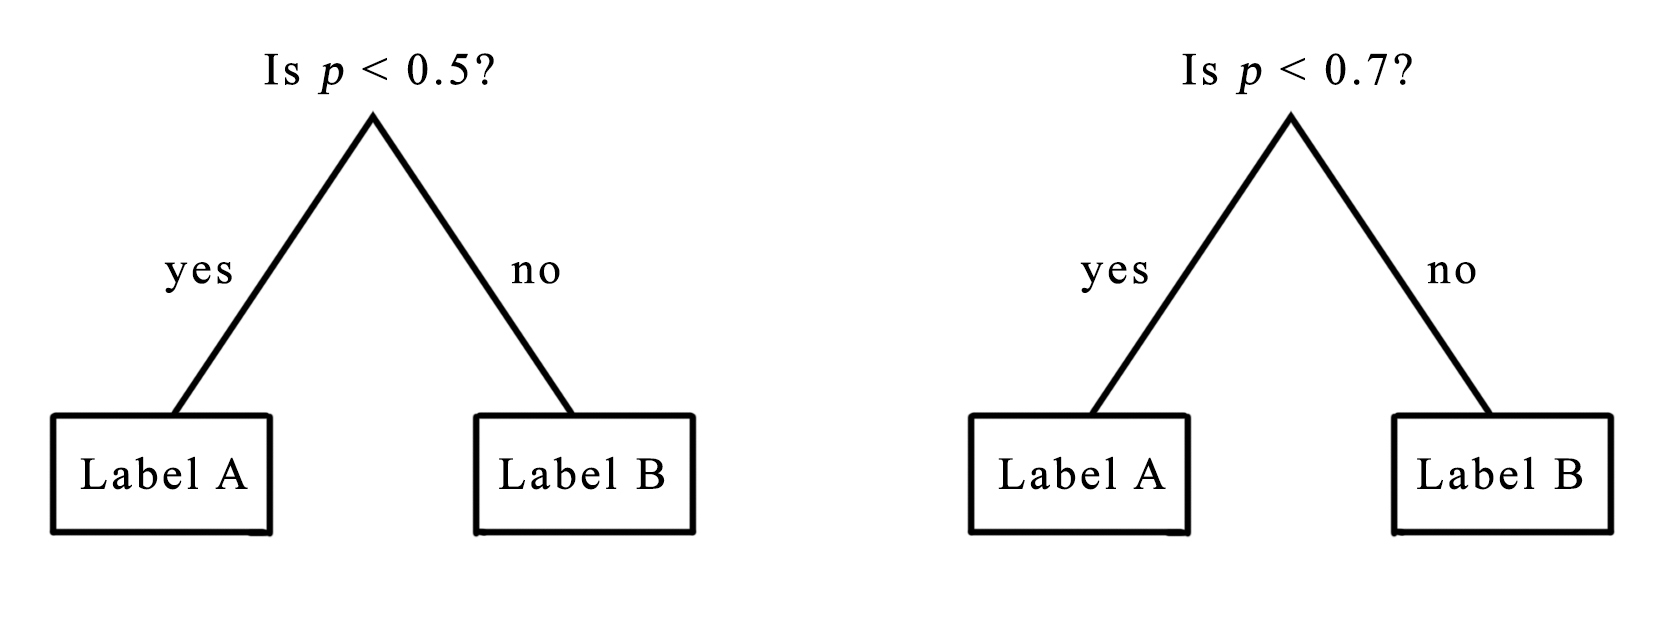
\includegraphics[width=0.75\linewidth]{ch-visualizer/figures/tree}
		\caption[Classifiers and classification models]{Although both figures 
		on the left and right are slightly different classifiers, they 
		are both instances of (extremely simple) decision trees.}
		\label{fig:visualizer:al:tree}
	\end{center}
\end{figure}

\subsection{Initialization of active learner}
\label{sec:visualizer:al:initialization}

It is problematic to start from scratch; how does the system determine
the best first point of ambiguity when it knows nothing (the hypothesis space is
everything)? A classic method is to simply select $k$ random data instances for 
the user to label. As initialization is not the focus of this work, the VS 
currently utilizes this methodology.

Alternatively, we can exploit the fact that the
user is already providing a numerical model that they believe to be a good
representation of the data which they would like the visualization system to
check visually. Given this data, the system builds a decision tree that utilizes
the various properties of the plots to determine whether one is interesting or
uninteresting. Doing so greatly narrows the hypothesis space and makes it easier
to determine points of ambiguity. However, to reconcile with the fact that the
user wishes to check the numerical model and may not necessarily believe it is a
good representation of fit, the learner must check whether the initial decision
tree is a proper fit (This may be achieved with line-up tests, which are 
described briefly in Section ~\ref{sec:futurework:lineup}). As the user then 
proceeds to label various conditional
plots as ``interesting'' or ``not interesting,'' the classifier learns the
user’s interest and continues to evolve. This models plot characteristics that
the user found interesting to study.

\subsection{Decision tree classification of user interests}
\label{sec:visualizer:al:tree}

Post-initialization, the active learner cleverly queries vital plots so that 
the system can best learn the user’s interests. The system first determines 
which features it is uncertain about classifying and then returns a plot 
matching those characteristics to the user. This allows the system to utilize 
its classification model of choice to build a better classifier more 
efficiently. It is important to distinguish between the active learner, which 
selects the next queries from the pool of unlabeled data, and the
classification model, which trains on labeled data to ``learn'' user interests 
and classify (predict) the remaining unlabeled data. 

A random forest is one model for classifying and labeling data (features of 
plots, in the case of the visualization system). In a random forest, various 
decision trees are constructed from random samples of the data. Each classifier 
has a vote of weight one for each unlabeled data, and the forest is aggregated 
by majority vote. It is easily presented to the 
analyst in the form of a decision tree, which aids in user 
interpretability of the system output. As such, the VS sets the choice of 
classification model to random forest by default.
